
\chapter{Machine Learning Theory}
\label{ch:ML_theory}

\epigraph{\textit{``People worry that computers will get too smart and take over the world, but the real problem is that they're too stupid and they've already taken over the world.''}}{--- Pedro Domingos}

\newthought{Machine Learning} is the method of teaching computers how to automatically find patterns in (often high-dimensional) data. According to some sceptics machine learning (ML) is just glorified statistics, however, by the same logic physics is just glorified mathematics. In contrary, machine learning is a collection of different subjects located somewhere along the hypothetical line from simple, classical statistics to futuristic artificial intelligence. It includes methods ranging from the well-known statistical methods such as linear regression to the modern, advanced zoo of different neural networks \citep{veenNeuralNetworkZoo2016} which has seen a plethora of use cases in recent years. 

\section{Statistical Learning Theory}
This chapter deals with the theory of ML which Statistical Learning Theory is a subcategory of. Many books are written on the subject where this thesis especially follows the overall notation used in the very accessible introduction in the book Learning From Data \citep{abu-mostafaLearningData2012} and the graduate course Advanced Topics in Machine Learning \citep{AdvancedTopicsMachine} at the computer science institute\sidenote{Datalogisk Institut Københavns Universitet, DIKU.} at the faculty of Science, University of Copenhagen. Statistical learning theory is the analysis of how to not only find the function, or \emph{hypothesis}, that matches the data best, but also bounding the difference in performance between this hypothesis and the hidden, underlying data generation distribution often only known by Nature. 

Overall there are two main branches within machine learning: \emph{supervised} and \emph{unsupervised}\sidenote{Also known as \q{self-supervised} or \q{predictive} learning.}. The difference depends on whether or not the data that is trained on is labelled or not. Classic linear regression is an example of the former and linear dimensionality reduction using PCA of the latter. Since unsupervised learning techniques are only used sparsely throughout this project, the main focus will be on supervised learning. 

\section{Supervised Learning}
\label{sec:ml:supervised_learning}
In supervised learning we are given a set of $N$ different samples of which we for each one knows $M$ different variables written as the column-vector $\vec{x}_i = [x_1, x_2, \dots, x_M]^T \in \mathcal{X}$ for the $i$th observation and $\mathcal{X}$ denotes the sample space. All of these samples as a whole is written as the matrix $\vec{X}$ with the individual observations $\vec{x}_i$ transposed and stacked on top of each other $\vec{X} = [\vec{x}_0^T, \vec{x}_1^T, \dots, \vec{x}_N^T]$ such that row $i$ in $\vec{X}$ corresponds to observation $i$. In the case of supervised learning we also have the label $y$ of each sample $y \in \mathcal{Y}$ where $\mathcal{Y}$ denotes the label space. 
In the case where $y$ is a real number $\mathcal{Y} = \mathbb{R}$ the problem is said to a \emph{regression} problem, e.g. predicting the price of a house. On the contrary, if $\mathcal{Y}$ is binary such that $\mathcal{Y} = \{0, 1\}$ then the problem is said to be a (binary) \emph{classification} problem\sidenote{If $\mathcal{Y}\subset \mathbb{Z}$ then it would be a multiclass classification problem.} e.g. predicting whether or not a particle is a quark or not. 

\begin{marginfigure}
  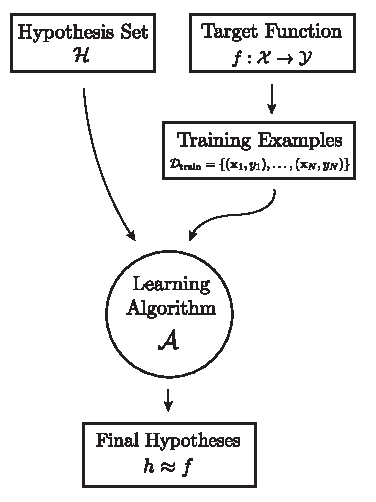
\includegraphics[width=0.99\textwidth]{figures/learning_problem/learning_problem.pdf}
  \caption[The Learning Problem]
    {Schematic overview of the learning problem and how to find the optimal hypothesis $h^*$ to approximate $f$ given the training data $\mathcal{D}_\mathrm{train}$.
    }
  \label{fig:ml:learning_problem}
\end{marginfigure}

Without any loss of generality let the focus for now be on classification. The goal is to find the underlying \q{true} function $f: \mathcal{X} \mapsto \mathcal{Y}$ that gives the correct label $y$ for each observation $\vec{x}$. This function, however, is unknown and cannot perfectly be found. Although it is impossible to find $f$ it is possible to learn an approximation of it, $h$, based on some training observations $\mathcal{D}_\mathrm{train} = \left \{(\vec{x}_1, y_1), \dots, (\vec{x}_N, y_N) \right\}$. The optimal hypothesis, $h^*$, is chosen among a set of $K$ candidate hypotheses $\mathcal{H} = \left\{h_1, h_2, \ldots, h_K  \right\}$, and hopefully $h^*$ will be a good approximation of $f$: $h^* \approx f$. A schematic overview of this process can be seen in Figure~\ref{fig:ml:learning_problem}. 

How can one make sure that $h^*$ really is a good approximation of $f$? That is where statistical learning theory comes into play. From a statistical standpoint we are interested in modelling the unknown joint probability $P(\vec{x}, y)$ over $\mathcal{X}$ and $\mathcal{Y}$. We assume that $\mathcal{D}_\mathrm{train}$ is independent and identically distributed (\emph{iid})\sidenote{This is one of the two key assumptions of statistical learning theory, the other being that future events are coming from the same distrubution as the one that generated the past events. These assumptions are sometimes called the \emph{PAC} assumptions where PAC is an abbreviation for Probably, Approximately Correct.} from $P(\vec{x}, y)$ and thus want to find the hypothesis whose predictions $h(\vec{x})=\hat{y}$ matches the conditional probability distribution $P(y|\vec{x})$ as well as possible. 

To quantify the statement \q{as well as possible} in the previous paragraph, we define the loss function $\ell$ which measures the loss for predicting $\hat{y}$ instead of $y$: $\ell(\hat{y}, y) = \ell(h(\vec{x}), y) \in \mathbb{R}^+$. Given $\ell$ we now introduce the method of (empirical) risk minimization \citep{vapnikPrinciplesRiskMinimization1991} and the expected loss\sidenote{Also called expected error or the out-of-sample error.}:
\begin{equation} 
  \label{eq:L}
  L(h) = \mathbb{E} \left[\ell(h(\vec{x}), y) \right] = \int \ell(h(\vec{x}), y)  \, dP(\vec{x}, y).
  \end{equation}
The optimal hypotheses $h^*$ is the hypothesis which minimizes the expected loss $L(h)$. However, the joint probability distribution $P(\vec{x}, y)$ is unknown and we are thus left with the empirical loss\sidenote{Also called empirical error.} of $h$ on $\mathcal{D}_\mathrm{train}$:
\begin{equation}
  \label{eq:L_hat}
  \hat{L}(h, S) = \frac{1}{N} \sum_{i=1}^{N} \ell(h(\vec{x}_i), y_i), % \equiv \mathcal{L} 
\end{equation}
which is an approximation of $L(h)$ based on the training data available. 
% In the remainder of the text $\hat{L}(h, S)$ and $\mathcal{L}$ will be used interchangeably. 
Now the optimal hypothesis $h^*$ can defined:
\begin{equation}
  h^* = \argmin_{h\in\mathcal{H}} \hat{L}(h, S).
\end{equation}

\section{Generalization Bound}
\label{sec:generalization_bound}
In \autoref{sec:ml:supervised_learning} the method of selecting the optimal hypotheses $h^*$ out of the total set of candidate hypothesis $\mathcal{H}$ was sketched. However, there is still no guarantee that $h^*$ will work well, that is to say that the \emph{generalization error} $G(h)$ might be big:
\begin{equation}
  G(h) = \hat{L}(h, S) - L(h).
\end{equation}
The generalization error is thus the difference between the expected error $L(h)$ and the empirical error $\hat{L}(h, S)$. It describes the loss in performance of our chosen model compared to the optimal, yet hidden, model. Since $P(\vec{x}, y)$ is unknown, $G(h)$ cannot be computed, however, it is possible to bound this error using statistical learning theory. To do so, the union bound and Hoeffding's (one-sided) inequalities are introduced. 
\begin{lemma}[The Union Bound]
  For any finite or countably infinite sequence of events $E_1, E_2, \dots$ (not necessarily independent): 
  \begin{equation}
    \mathbb{P} \left\{\bigcup_{1 \leq i} E_i \right\} \leq \sum_{1 \leq i} \mathbb{P} \left\{E_i \right \}. 
  \end{equation}
\end{lemma}
The union bound, in simple terms, states that the probability of any one of $n$ events happening is less than or equal to the sum of the individual probabilities of the events happening. As an example, let $E_1=\{2, 4, 6\}$ be the event that a die rolls an even number and $E_2=\{4, 5, 6\}$ be the event that a die rolls a number larger than or equal to $4$. Then $\mathbb{P} \left\{E_1 \cup E_2 \right\} = \mathbb{P} \left\{ 2, 4, 5, 6 \right\} \leq \mathbb{P} \left\{E_1 \right \} + \mathbb{P} \left\{E_2 \right \} $. 
\begin{lemma}[The one-sided Hoeffding's inequalities]
  Let $Z_1, \dots, Z_N$ be independent random variables each belonging to the $[0, 1]$ interval such that $\mathbb{P}\left\{Z_i \in [0, 1] \right\} = 1$ and $\mathbb{E}[Z_i] = \mu$ for all i, then for every $\epsilon > 0$:
  \begin{equation}
    \mathbb{P} \left\{  \frac{1}{N}\sum_{i=1}^N Z_i - \mu \geq \epsilon \right\} \leq e^{-2N\epsilon^2} 
    \label{eq:hoeffding_onesided_a}
  \end{equation}
  and
  \begin{equation}
    \mathbb{P} \left\{ \mu - \frac{1}{N}\sum_{i=1}^N Z_i  \geq \epsilon \right\} \leq e^{-2N\epsilon^2}.
    \label{eq:hoeffding_onesided_b}
  \end{equation}
\end{lemma}
When using the union bound on equation \eqref{eq:hoeffding_onesided_a} and equation \eqref{eq:hoeffding_onesided_b} we arrive at Hoeffding's (two) sided inequality:
\begin{lemma}[The two-sided Hoeffding's inequality]
  \label{lemma:hoeffding}
  Let $Z_1, \dots, Z_N$ be independent random variables each belonging to the $[0, 1]$ interval such that $\mathbb{P}\left\{Z_i \in [0, 1] \right\} = 1$ and $\mathbb{E}[Z_i] = \mu$ for all i, then for every $\epsilon > 0$:
  \begin{equation}
    \mathbb{P} \left\{ \left| \frac{1}{N}\sum_{i=1}^n Z_i - \mu \right| \geq \epsilon \right\} \equiv \mathbb{P} \left\{ \left| \hat{\mu} - \mu \right| \geq \epsilon \right\} \leq 2 e^{-2N\epsilon^2},
    \label{eq:hoeffding_inequality}
  \end{equation}
  where we have defined the empirical average of $Z$ to be $\hat{\mu}$: $\hat{\mu}=\frac{1}{n}\sum_{i=1}^N Z_i $
\end{lemma}
Assuming that the loss $\ell(\hat{y}, y)$ is bounded in the $[0, 1]$ interval\sidenote{Which it is for classification, however, it can be extended in a similar fashion for regression.}, $\ell(\hat{y}, y) \in [0, 1]$ for all $(\hat{y} y)$, we can bound the generalization error $G(h)$ by letting $Z_i = \ell(\hat{y}_i, y_i) = \ell(h(\vec{x}_i), y_i)$ be the loss of $h$ in sample $(\vec{x}_i, y_i)$. By comparing Lemma \ref{lemma:hoeffding} and equation \eqref{eq:L_hat} we see that $\hat{\mu} = \hat{L}(h, S)$, and similar for equation \eqref{eq:L}: $\mu = L(h)$. We then see that the generalization error is bounded:
\begin{equation}
  \label{eq:hoeffding_inequality_generalization_error}
  \mathbb{P} \left\{ \left| G(h) \right| \geq \epsilon \right\} = \mathbb{P} \left\{ \left| \hat{L}(h, S) - L(h) \right| \geq \epsilon \right\} \leq 2 e^{-2N\epsilon^2}.
\end{equation}
This equation provides a bound on the difference between the empirical loss and the expected loss. 
% Say the probability of the generalization error being larger than $\epsilon = 0.1$ is needed for $N=100$ samples, we find that the this probability is $P=27\%$. 
The generalization bound  can be rewritten in terms of $\delta$:
\begin{equation}
  \delta \equiv 2 e^{-2N\epsilon^2} \in (0, 1) \quad \Rightarrow \quad \epsilon = \sqrt{\frac{\ln \frac{2}{\delta}}{2N}}.
\end{equation}
\begin{theorem}[Hoeffding's inequality for a single hypothesis]
  \label{theorem:hoeffding_single}
  Assume that $\ell$ if bounded in the $[0, 1]$ interval, then for a single hypothesis $h$ and any $\delta\in(0,1)$ we have:  
  \begin{equation}
    \label{eq:hoeffding_inequality_generalization_error_delta}
    \mathbb{P} \left\{ \left| \hat{L}(h, S) - L(h) \right| \geq \sqrt{\frac{\ln \frac{2}{\delta}}{2N}}  \right\} \leq \delta.
  \end{equation}
\end{theorem}
Equation \eqref{eq:hoeffding_inequality_generalization_error_delta} can be read as the probability of the generalization error being larger than $\sqrt{\frac{\ln \frac{2}{\delta}}{2N}}$ is $\delta$ or less, or, similarly, that with probability greater than $1-\delta$:
\begin{equation}
  \label{eq:hoeffding_inequality_single_PAC}
  \left| \hat{L}(h, S) - L(h) \right| \leq \sqrt{\frac{\ln \frac{2}{\delta}}{2N}}.
\end{equation}
This is a powerful result relating the performance for a (fixed) hypothesis $h$ with the number of samples, $N$. We see that a higher $N$ yields a tighter bound on the generalization error.
% inversely\sidenote{Not to be understood as $1/x$ in this context.} related to on the certainty\sidenote{Technically the certainty of the model is $1-\delta$.} $\delta$ of this bound.

There is a big assumption of this derivation: that the hypothesis $h$ cannot depend on the sample $S$ and thus has to be chosen before seeing the data. We say that $h$ has to be \emph{fixed}. Of course the term machine learning indicates that some kind of learning is taking place: exactly as seen previously where we wanted to find the optimal hypotheses $h^*$ out of all the possible ones $\mathcal{H}$. For now assume that $\mathcal{H}$ is finite and consists of $K$ hypotheses: $|\mathcal{H}| = K$. We thus have $[h_1, h_2, \dots, h_K]$ hypotheses which we test simultaneously and where Hoeffding's inequality is true for each of them leading to the following theorem:
\begin{theorem}[Hoeffding's inequality for a finite set of hypotheses candidates]
  \label{theorem:hoeffding_finite}
  Assume that $\ell$ is bounded in the $[0, 1]$ interval and that $|\mathcal{H}| = K$. Then for any $\delta\in(0,1)$ we have:  
  \begin{equation}
    \label{eq:hoeffding_inequality_theorem_multiple}
    \mathbb{P} \left\{ \exists h \in \mathcal{H}: \left| \hat{L}(h, S) - L(h) \right| \geq \sqrt{\frac{\ln \frac{2K}{\delta}}{2N}}  \right\} \leq \delta.
  \end{equation}
\end{theorem}

\begin{proof}
  The proof begins by denoting $h_i$ as the event where: 
  \begin{equation*}
    \left| \hat{L}(h_i, S) - L(h_i) \right| \geq \sqrt{\frac{\ln \frac{2}{\delta'}}{2N}},
  \end{equation*}
   and then taking the union bound (the first inequality below) followed by applying Hoeffding's inequality to each part in the sum (the second inequality): 
\begin{equation*}
  % \label{eq:hoeffding_inequality_generalization_error_delta}
  \begin{split}
    \mathbb{P} \Biggl\{ \exists h \in \mathcal{H}: \left| \hat{L}(h, S) - L(h) \right| &\geq \sqrt{\frac{\ln \frac{2}{\delta'}}{2N}}  \Biggr\} \\
    &= \mathbb{P} \left\{ \bigcup_{h \in \mathcal{H}} \left| \hat{L}(h, S) - L(h) \right| \geq \sqrt{\frac{\ln \frac{2}{\delta'}}{2N}}  \right\}  \\
    &\leq \sum_{h \in \mathcal{H}} \mathbb{P} \left\{\left| \hat{L}(h, S) - L(h) \right| \geq \sqrt{\frac{\ln \frac{2}{\delta'}}{2N}} \right\}  \\
    &\leq \sum_{h \in \mathcal{H}} \delta' \\
    &= K \delta'.
  \end{split}
\end{equation*}
By making the substitution $\delta = K \delta'$ we arrive at equation \eqref{eq:hoeffding_inequality_theorem_multiple}. 
\end{proof}

As we did in equation \eqref{eq:hoeffding_inequality_single_PAC}, equation \eqref{eq:hoeffding_inequality_theorem_multiple} can also be read as with probability greater than $1-\delta$ then for all $h\in\mathcal{H}$:
\begin{equation}
  \label{eq:hoeffding_inequality_multi_PAC}
  \left| \hat{L}(h, S) - L(h) \right| \leq \sqrt{\frac{\ln \frac{2K}{\delta}}{2N}}.
\end{equation}
This bound is looser than the one for only a single hypothesis by a factor $\ln K$, however, this holds for the optimal hypothesis $h^*$. 

\subsection{Generalization Bound for Infinite Hypotheses}
\label{subsec:generalization_bound_infinite}
Section \ref{sec:generalization_bound} dealt with the case of a single hypotheses $h$ and a finite set of candidate hypotheses $h\in\mathcal{H}, |\mathcal{H}| = K$. When $K$ goes towards infinity the generalization bound goes to infinity and the bound becomes useless. However, even simple models such as a linear classifier\sidenote{Also known as the perceptron. Often includes a constant offset $b$ as well which is omitted here for brevity. The functional form of this function is $f(x)=\mathrm{sign}(\vec{w}^T\vec{x})$.} that predicts $\hat{y}=1$ when the dot product $\vec{w}^T\vec{x}$ is positive and $\hat{y}=-1$ when it is negative, has $|\mathcal{H}| = \infty$. Since an infinite number of hypotheses $h(\vec{w})$ exists, assuming we allow $\vec{w}$ to take any real values as is almost always the case, $\mathcal{H}$ is infinite. 

To solve this obvious problem with the Hoeffding inequality, we introduce\sidenote{For proof, see: \citet{abu-mostafaLearningData2012}} the Vapnik-Chervonenkis (VC) generalization bound. The VC-bound is based on the so-called VC-dimension of the hypothesis space $\mathcal{H}$: $d_\mathrm{VC}(\mathcal{H}) = d_\mathrm{VC}$. The VC-dimension is a measure of the complexity of the hypothesis space, the degrees of freedom of the model so to say. For example the VC-dimension of the $M$-dimensional linear classifier defined above\sidenote{In the general case when the offset $b$ is included: $d_\mathrm{VC}=M+1$.} is $d_\mathrm{VC}=M$ for $\{\vec{x}, \vec{w}\} \in \mathbb{R}^M$. 
\begin{theorem}[VC Generalization Bound]
  \label{theorem:VC_generalization_bound}
  Let $\mathcal{H}$ be a hypotheses class with VC-dimension: $d_\mathrm{VC}(\mathcal{H}) = d_\mathrm{VC}$. Then with probability at least $1-\delta$: 
  \begin{equation}
    \label{eq:VC_bound}
    L(h) \leq \hat{L}(h, S) + \sqrt{ \frac{8}{N} \ln \left( \frac{4}{\delta} \left( \left(2N \right)^{d_\mathrm{VC}} + 1 \right)  \right)} .
  \end{equation}
\end{theorem}
Equation \eqref{eq:VC_bound} states that the out of sample error $L(h)$ is bounded from above by the empirical error $\hat{L}(h, S)$ and the $\sqrt{ \boldsymbol{\cdot}}$ which is related to the complexity of the hypothesis space $\mathcal{H}$, the number of samples $N$ and the certainty $\delta$. We will call this model complexity penalty $\Omega(N, \mathcal{H}, \delta)$:
\begin{equation}
  \Omega(N, \mathcal{H}, \delta) = \sqrt{ \frac{8}{N} \ln \left( \frac{4}{\delta} \left( \left(2N \right)^{d_\mathrm{VC}(\mathcal{H})} + 1 \right)  \right)}.
\end{equation}
As the hypothesis space complexity $d_\mathrm{VC}$ grows, the model complexity penalty increases but it is more likely that $\mathcal{H}$ contains a strong hypothesis. This relationship is called the approximation-estimation or the  \emph{bias-variance} tradeoff. When the model is too simple to properly fit the complexity in the data it is called \emph{underfitting}\sidenote{Here the error from $\hat{L}(h, S)$ dominates.}, when the model is so complex that it starts fitting the inherent noise in the data it is called \emph{overfitting}\sidenote{Here the error from $\Omega(N, \mathcal{H}, \delta)$ dominates.}. The loss as a function of model complexity gives the characteristic curve illustrated in Figure~\ref{fig:ml:empirical_risk}. As the model complexity increases the training loss decreases. Initially also the validation loss decreases, but at some point the behavior of model on the validation set worsens and the loss increases; overfitting happens. 

\begin{marginfigure}
  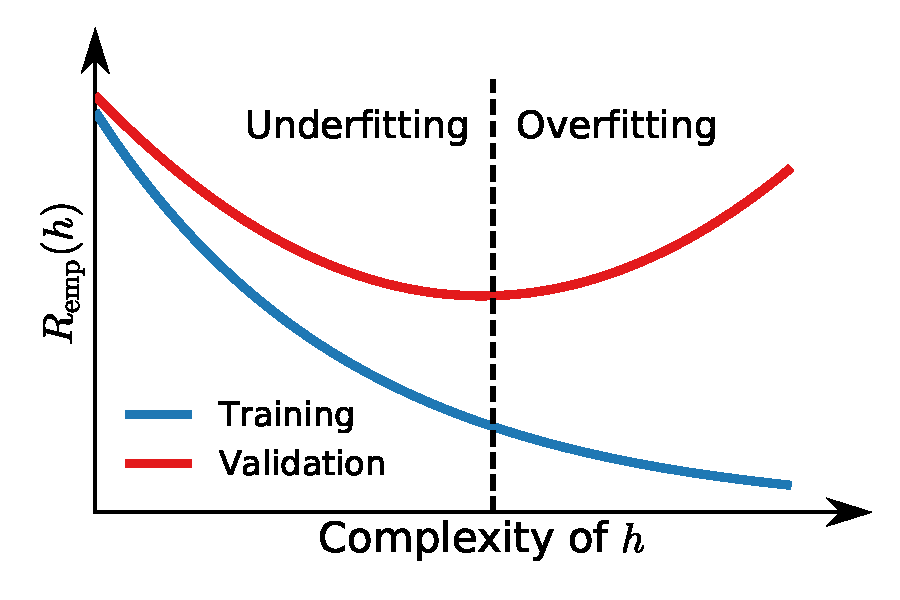
\includegraphics[width=0.98\textwidth]{figures/overfitting/overfitting_1.pdf}
  \caption[Approximation-Estimation Tradeoff]
    {Illustration of the empirical loss as a function of model complexity. The \textcolor{blue}{training error} is shown in blue and \textcolor{red}{validation error} in red.
    }
  \label{fig:ml:empirical_risk}
\end{marginfigure}


\section{Avoiding overfitting}
\label{sec:ml:overfitting}
Avoiding overfitting is one of the most important issues in machine learning. By now, most modern machine learning algorithms have the inherent model complexity needed for overfitting and thus it has to be managed. Due to the importance of the issue, a number of different methods preventing or reducing overfitting exists. Most of them are complementary of each other but can be taken advantage of in a combination. In this section model regularization will be introduced in \autoref{subsec:regularization}, cross validation in \autoref{subsec:cross_validation}, and early stopping in \autoref{subsec:early_stopping}. 

\subsection{Model Regularization}
\label{subsec:regularization}
One of the earliest methods developed for preventing overfitting was model regularization. A. N. Tikhonov \citep{tikhonovStabilityInverseProblems1943} was one of the first to describe this method in \num{1943}. In particular, regularization was used to solve \emph{ill posed} linear regression problems. Regular linear regression problems refer to minimizing the residual sum of squares written in matrix form as:
\begin{equation}
  \begin{split}
    \hat{\bm{\beta}}_{\mathrm{LS}} = \argmin_{\bm{\beta}} \norm{\vec{y} - \vec{X} \bm{\beta} }_2^2 = \argmin_{\bm{\beta}} \norm{ \vec{y} - \vec{f}(\vec{X}) }_2^2 \\
    \vec{f}(\vec{X}) = \vec{X} \bm{\beta},
  \end{split}
\end{equation}
where $\vec{y}$ is the vector of values we are trying to predict\sidenote{E.g. the prices of a collection of houses.}, $\vec{X}\in\mathbb{R}^{N\times M}$ the matrix of input variables, $\hat{\bm{\beta}}_{\mathrm{LS}}$ the vector of unknown coefficients\sidenote{Here excluding the constant offset $\beta_0$ which can be included trivially.} of the linear least squares (LS) model $\vec{f}$, and $\norm{ \bm{\cdot} }_2$ is the normal Euclidean norm. In general, the $p$-norm is defined as:
\begin{equation}
  \norm{\vec{x}}_p = \left( \sum_{i=1}^N \abs{x_i}^p \right)^{1/p}.
\end{equation}
Differentiating the objective $\norm{\vec{y} - \vec{X} \bm{\beta} }_2^2$ with respect to (w.r.t.) $\bm{\beta}$ and setting the derivative equal to $0$ to find the minimum\sidenote{When checking the double derivative wrt. $\bm{\beta}$ it is seen that this really is a minimum and not a maximum (or saddle point).} yields the solution for $\bm{\beta}$:
\begin{equation}
  \begin{split}
    \frac{\partial}{\partial \bm{\beta}} \norm{\vec{y} - \vec{X} \bm{\beta} }_2^2 = -2 \vec{X}^T \left( \vec{y} - \vec{X} \bm{\beta} \right) = 0  \Rightarrow \\
    \vec{X}^T \vec{y} - \vec{X}^T \vec{X} \bm{\beta} \Rightarrow \\
    \hat{\bm{\beta}}_{\mathrm{LS}} =  \left( \vec{X}^T \vec{X} \right)^{-1} \vec{X}^T \vec{y}.
  \end{split}
\end{equation}
However, this solution for $\hat{\bm{\beta}}_{\mathrm{LS}}$ is only valid when $\vec{X}^T \vec{X}$ is invertible, i.e. $\vec{X}$ has to be full rank \citep{hastieElementsStatisticalLearning2009}. If this is not the case, the problem is said to be ill posed. Tikhonov solved this problem by adding an extra term to the minimization problem, which we will call $\Omega$ for simplicity. For a specific choice of $\Omega$, one gets:
\begin{equation}
  \label{eq:l2_norm}
  \hat{\bm{\beta}}_{\mathrm{L_2}} = \argmin_{\bm{\beta}} \left \{\norm{ \vec{y} - \vec{f}(\vec{X}) }_2^2 + \lambda \norm{ \bm{\beta} }^2_2 \right \},
\end{equation}
where $\lambda \geq 0$ is the regularization strength. This is the so-called $L_2$-regularization, also known as ridge regression for linear problems. For ridge regression\sidenote{Here $\hat{\bm{\beta}}_{\mathrm{L_2}}$ is the solution for any general function $\vec{f}$ and $\hat{\bm{\beta}}_{\mathrm{ridge}}$ is the specific solution for a linear function $\vec{f}$, where linear is w.r.t. to the model parameters $\bm{\beta}$.} the corresponding solution for $\bm{\beta}$ is:
\begin{equation}
  \label{eq:l2_norm_linear}
  \hat{\bm{\beta}}_{\mathrm{ridge}} =  \left( \vec{X}^T \vec{X} + \lambda \vec{I} \right)^{-1} \vec{X}^T \vec{y},
\end{equation}
where $\vec{I}$ is the identity matrix\sidenote{The $\lambda \vec{I}$ in equation \eqref{eq:l2_norm_linear} also acts as a conditioner on the problem in the sense that it reduces the condition number of the matrix to be inverted turning the ill-posed problem to a well-behaved one.}. This extra term, $\Omega =  \lambda \norm{ \bm{\beta} }^2_2$, acts as a shrinkage factor on the coefficients of $\bm{\beta}$. Looking at equation \eqref{eq:l2_norm}, we see that this is the Lagrangian form of the equivalent problem: 
\begin{equation}
  % \label{eq:ml:constrained_minimization_L2}
  \begin{split}
    \hat{\bm{\beta}}_{\mathrm{L_2}} = \argmin_{\bm{\beta}} \norm{ \vec{y} - \vec{f}(\vec{X}) }_2^2 \\
    \mathrm{subject~to:} \quad \sum_{i=1}^N \beta_i^2 = \norm{\bm{\beta}}^2_2 \leq t,
  \end{split}
  \label{eq:l2_norm_non_lagrangian}
\end{equation}

for some $t \geq 0$ with a one-to-one mapping between $\lambda$ and $t$. We thus see that $L_2$ regularizes the coefficients of $\bm{\beta}$ to have some maximal norm. The effect of the regularization is controlled by $\lambda$, where $\hat{\bm{\beta}}_{\mathrm{L_2}} \rightarrow \hat{\bm{\beta}}_{\mathrm{LS}}$ for $\lambda \rightarrow 0$ and $\hat{\bm{\beta}}_{\mathrm{L_2}} \rightarrow \vec{0}$ for $\lambda \rightarrow \infty$. An example of this can be seen in Figure~\ref{fig:ml:regularization_ridge}. 
\begin{marginfigure}
  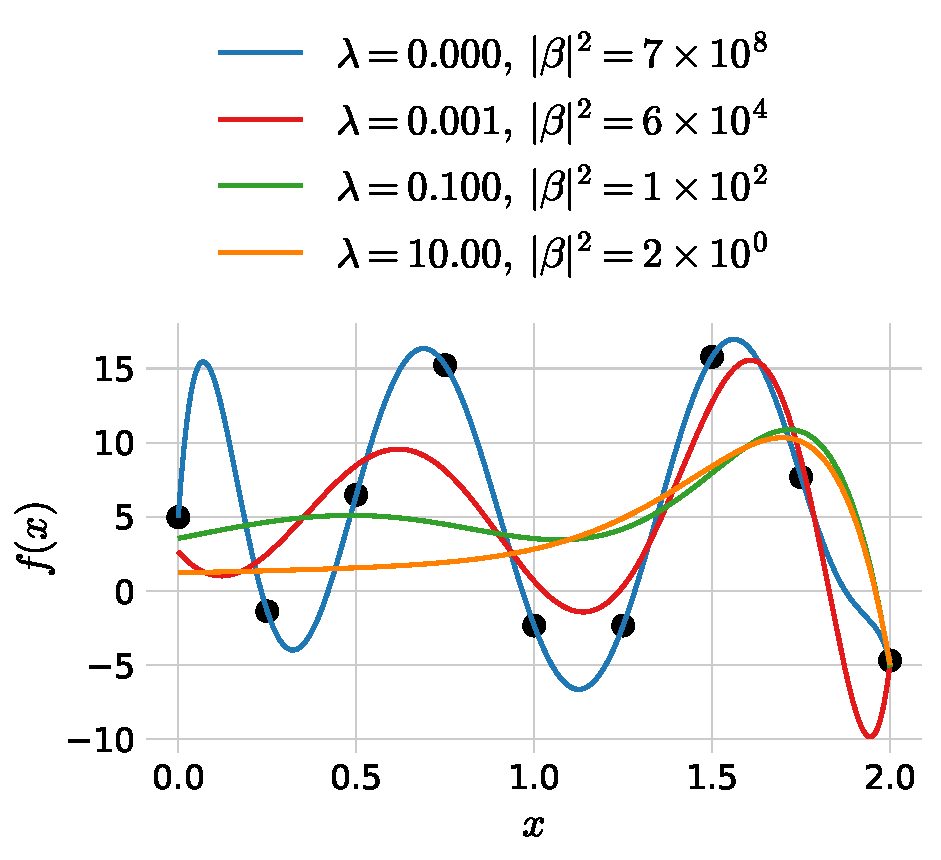
\includegraphics[width=0.99\textwidth, trim=5 5 5 5, clip]{figures/ridge_regression/ridge.pdf}
  \caption[Regularization Strength]
    {Effect of tuning the regularization strength $\lambda$ in ridge regression.
    }
  \label{fig:ml:regularization_ridge}
\end{marginfigure}
Here $N=9$ datapoints were randomly generated such that the $x$-values are evenly spaced from \num{0} to \num{2} and $y \sim \mathcal{N}(\mu=0, \sigma=10)$. They were then fit with a \num{9}-order polynomial by minimizing equation \eqref{eq:l2_norm} for different values of $\lambda$. Here we see the regularizing effect of $\lambda$, going from $\lambda=0$ in blue which fits all points\sidenote{Since the order of the polynomial is the same as the number of datapoints.} with a high degree of variance and a wildly oscillatory pattern to $\lambda=10$ in orange which is mostly flat in most of the interval. Also note in the legend how the norm of the fit parameters also decrease with $\lambda$ as expected. This is a great example of the \emph{bias-variance} tradeoff mentioned in \autoref{subsec:generalization_bound_infinite}, where bias refers the error the model makes when it is not advanced enough to fit the overall trend in the data (underfitting) and variance refers to the error the model makes when it starts to fit spurious noisy fluctuations in the training set which are not present in the validation set (overfitting). In this example $\lambda=0$ is clearly overfitting the data whereas $\lambda=10$ is an example of underfitting. 

\begin{marginfigure}[-0.5cm]
  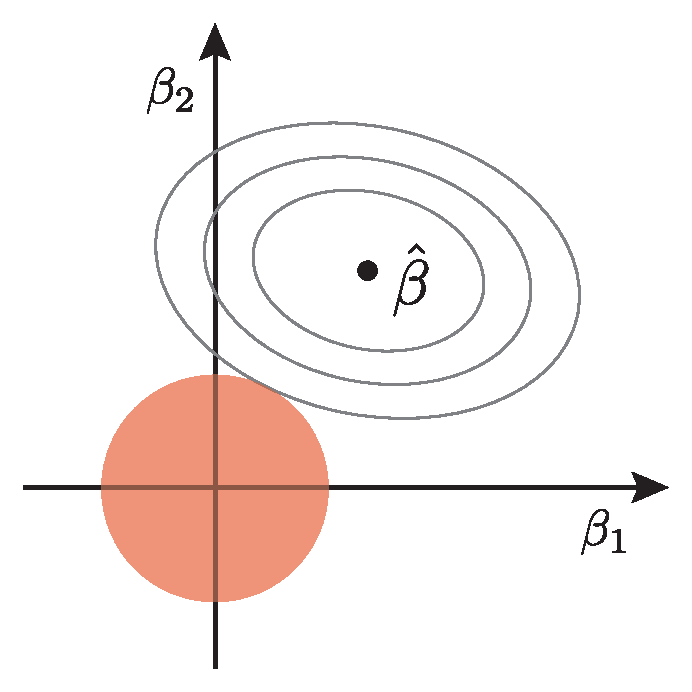
\includegraphics[width=0.7\textwidth]{figures/ridge_lasso_sparse/ridge.pdf}
  \caption[Regularization Effect of $L_2$ ]
    {Sketch of the minimization problem defined in equation \eqref{eq:l2_norm_non_lagrangian}, i.e. for a $L_2$-penalty. The \textcolor{red}{constrain region} shown in red is defined as $\beta_1^2 + \beta_2^2 \leq t$ for $L_2$ in $2D$-space and the contours of the unconstrained solution is shown with grey, dashed lines. 
    }
  \label{fig:ml:regularization_effect_ridge}
\end{marginfigure}

Other values of the regularization function $\Omega$ exists, for example the $L_1$-penalty:
\begin{equation}
  \Omega = \lambda \norm{\bm{\beta}}_1, 
\end{equation}
where the 1-norm, also known as Manhattan norm, is used. In the case of linear problems the $L_1$-penalty leads to Lasso regression introduced by \citet{tibshiraniRegressionShrinkageSelection1996} in \num{1996}. As with the $L_2$-penalty, the $L_1$-penalty also regularizes the coefficients of $\bm{\beta}$, however, this loss leads to sparse\sidenote{Meaning that a number of the $\beta_i$ coefficients are 0, the number depending on $\lambda$.} solutions. An illustration of this can be seen in Figure~\ref{fig:ml:regularization_effect_ridge} and Figure~\ref{fig:ml:regularization_effect_lasso} where the constraint regions of $\bm{\beta}$ is shown in red and the grey ellipses are the contours of the non-constrained problem. Notice how the intersection of the contour lines and the constrain region leads to $\beta_1 \neq 0, \beta_2 \neq 0$ for the $L_2$-penalty whereas it leads to the sparse solution $\beta_1=0, \beta_2 \neq 0$ for the $L_1$-penalty. This is a general pattern seen for $L_p$-penalties for $p \leq 1$ \autocite{hastieElementsStatisticalLearning2009}.

\begin{marginfigure}[0.5cm]
  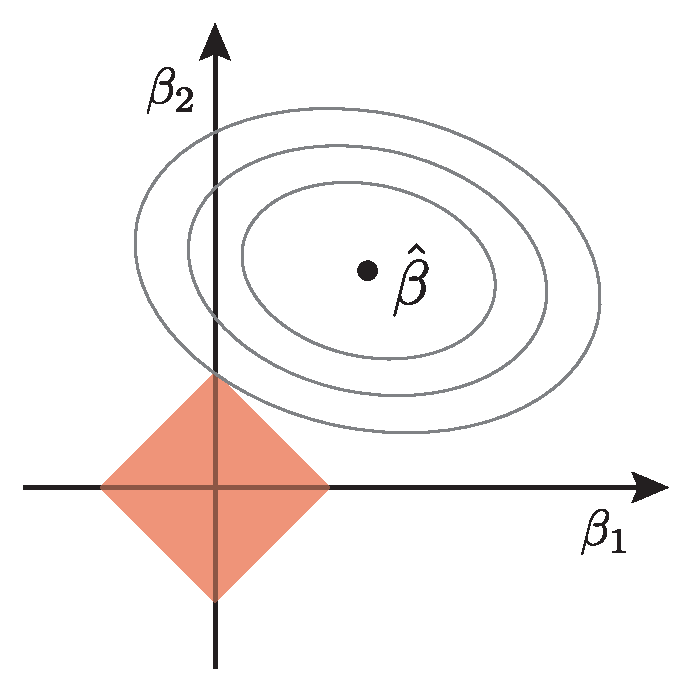
\includegraphics[width=0.7\textwidth]{figures/ridge_lasso_sparse/lasso.pdf}
  \caption[Regularization Effect of $L_1$]
    {Sketch of the similar minimization problem defined in Figure~\ref{fig:ml:regularization_effect_ridge} for the $L_1$-penalty. The \textcolor{red}{constrain region} shown in red is defined as $\abs{\beta_1} + \abs{\beta_2} \leq t$ for $L_1$ in $2D$-space and the contours of the unconstrained solution is shown with grey, dashed lines.
    }
  \label{fig:ml:regularization_effect_lasso}
\end{marginfigure} 

Overall, model regularization is heavily used in modern machine learning algorithms. In general, the function or the so-called \emph{objective function} $\mathcal{L}$ they are trying to minimize is:
\begin{equation}
  \mathcal{L}(h) = \hat{L}(\ell, h, S) + \Omega(h)
\end{equation}
where $\hat{L}$ is the empirical loss and $\Omega$ is the regularization penalty. As can be seen from the above discussion, choosing the right value for the regularization strength is fundamental problem in model regularization. How to choose a suitable value for $\lambda$ via cross validation is discussed in \autoref{subsec:cross_validation} and the choice of the training loss function $\ell$ in \autoref{sec:ml:loss_function}. 

\subsection{Cross Validation}
\label{subsec:cross_validation}
In general we want to  be able to estimate the performance\sidenote{\q{Performance} is used here as the word for the general metric to be optimized for, whether or not this metric should be maximized or minimized.} of the developed model. Since evaluating the model on the data it was already trained on would give a biased estimate of the performance, we need an unbiased method of doing so. The easiest way of doing so would be to set a fraction of the data aside, e.g. \SI{20}{\percent}, train on the remaining part and then evaluate the performance on the data set aside. Splitting the data up like this would provide us with a training (data)set and a test set in a $\num{80}:\num{20}$ ratio. This would then yield an unbiased performance estimate when evaluation the performance on the test set. 
However, if one then needed to compare two different models -- e.g. with different values of regularization strength $\lambda$ -- and choose the best one, as is often the case, this method would not work since we would choose the model with the best performance on the test set which can be seen as training on the test set and thus it has \q{tainted} the purity of the test set. To avoid this, an additional split is made such that we get a training set, a validation set, and a test set, where you often see a $\num{80}:\num{10}:\num{10}$ ratio. The two models can then be compared on the validation set and the performance of the chosen model can be estimated from the test set. 

\begin{marginfigure}
  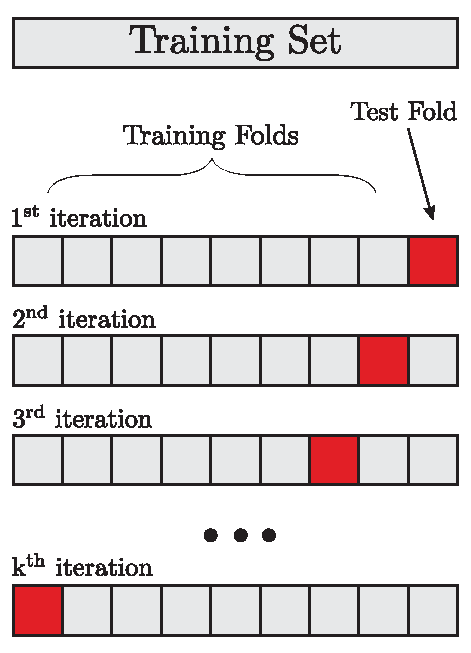
\includegraphics[width=0.98\textwidth, trim=5 5 5 5, clip]{figures/cross_validation/kfold.pdf}
  \caption[$k$-Fold Cross Validation]
    {$k$-fold cross validation. 
    }
  \label{fig:ml:cross_val_kfold}
\end{marginfigure} 

\begin{marginfigure}
  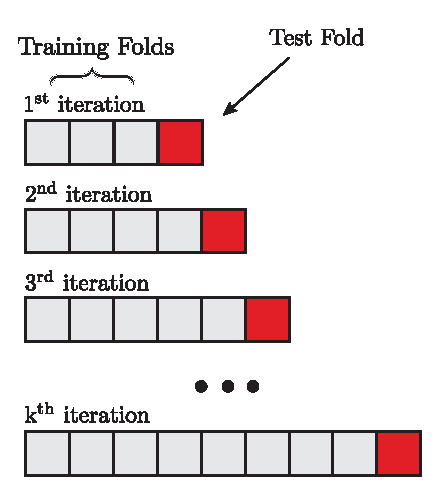
\includegraphics[width=0.98\textwidth, trim=10 10 10 10, clip]{figures/cross_validation/kfold_time.pdf}
  \caption[$k$-Fold Cross Validation for Time Series Data]
    {$k$-fold cross validation for time series data. 
    }
  \label{fig:ml:cross_val_kfold_time}
\end{marginfigure} 

This way of splitting up the data has some clear benefits and is thus also often used. There is a drawback, however, and that is that we are not fully utilizing a lot of the data in this way. Basically \SI{20}{\percent} of the data are only used to provide a single number of performance and does not necessarily allow an uncertainty or confidence interval of this measurement to be calculated. Thus other methods of estimating model performance are developed where one of the most used and well-known are the $k$-fold cross validation (CV). Here the entire dataset is split up into $k$ chunks which are randomly drawn subsamples (without replacement). In the first iteration, the model is trained on the first $k-1$ subsamples and evaluated on the last $k$ subsample. In the second iteration the evaluation subsample is a new one. This process is continued $k$ times until all samples in the dataset have been trained and evaluated on \citep{hastieElementsStatisticalLearning2009}. For an illustration of this, see Figure~\ref{fig:ml:cross_val_kfold}. The process yields $k$ estimates of the performance of the model which can then be averaged to form a single performance number and the variability of the performance can even be gauged\sidenote{Special care has to be taken here since the $k$ different performance values are not independent.}. The disadvantage of $k$-fold CV is that the performance estimate is now slightly biased, however, this effect is generally very small. The biggest disadvantage is the computational burden related to doing $k$-fold CV where $k\gg 1$. A compromise often used in applied machine learning is $k=5$ which is also what is used in this project.  

Special care has to be taken when dealing with time series data. Here the problem of \q{data leakage} is often introduced inadvertently. Data leakage is when the model is exposed to information from the test set that it was not supposed to be exposed to. In the case of time series data, if the data is split by the usual $k$-fold CV, then each subsample contains events from all times and the model does not learn how to predict future events. To circumvent this problem, a special type of $k$-fold CV for time series data has to be used. Here all samples up to a specific time, eg. all houses sold before 2018, is used for training and then the model is evaluated on the performance of samples after the event, e.g. houses sold in \num{2018}. For an illustration of this, see Figure~\ref{fig:ml:cross_val_kfold_time}.


\subsection{Early Stopping}
\label{subsec:early_stopping}
Most modern machine learning models are trained iteratively. This is the case for both (boosted) decision trees and neural networks, both of which are used in this project. Iteratively here means that the model starts off with an initial guess of the parameters of the model and then by looking at the data \q{learns} a new and better set of values. The question then become: for how long should the model be allowed to continue training?

This is a another example of the bias-variance tradeoff. The model should be trained long enough to be able to capture the complexity inherent in the data but also should not train for so long that it starts to overfit the data. Even though Figure~\ref{fig:ml:empirical_risk} was just an illustration of the bias variance tradeoff, it is also something that is seen in real data and can be taken advantage of through \emph{early stopping}. Early stopping is the process of monitoring the loss for the training set $\mathcal{D}_\mathrm{train}$ and validation set $\mathcal{D}_\mathrm{val}$. As mentioned in \autoref{subsec:cross_validation}, the model is only fitted on $\mathcal{D}_\mathrm{train}$ but the performance on $\mathcal{D}_\mathrm{val}$ is also measured. Whenever the validation loss starts to increase, the training of the model should be terminated. 

To avoid stopping due to a single noise-induced outlier which terminated the process, one often uses \emph{patience} in the early stopping process: if the loss has not decreased since the last minimum after \emph{patience} number of iterations, then terminate the process. Early stopping is thus an easy way of avoiding overfitting for iteratively trained models only requiring a validation set.  

\section{Loss functions}
\label{sec:ml:loss_function}
How we evaluate the performance of a model is of course very important since it defines the metric for the problem; what is good and what is bad? Obviously this depends on whether or not a classification problem or a regression problem is dealth with. Let us for know focus on the latter. Say that a house is estimated to cost \num{2} million DKK (\si{\Mkr}) but was sold for \SI{4}{\Mkr}. Compare this to a house that was estimated to cost \SI{8}{\Mkr} but was sold for \SI{6}{\Mkr} In both cases the price was \SI{2}{\Mkr} wrong, but does this mean that both predictions are equally good or bad? The first case was a factor of 2 off, whereas the prediction in the second case was only $33\%$ off compared to the true value. The first case underestimated the price whereas the second overestimated; should this have any importance?

As it should be clear by now the choice of loss function $\ell$ is of utmost importance. It is also not a problem that can be solved by computers, it is problem-specific, and has to be defined manually. The choice of loss function is what is called a \emph{hyperparameter}, the optimization of which is further discussed in \autoref{sec:ml:hyperparameter_optimization}. The most common choice of loss function is by far the Squared Error (SE): 
\begin{equation}
  \ell_\mathrm{SE}(y, \hat{y}) = \left( y-\hat{y} \right)^2,
\end{equation}
where $y$ is the true value and $\hat{y}$ is the predicted one. Squared Error has the advantage that it is differentiable everywhere, an effect that is both needed for many statistical derivations but also a requirement for some machine learning models. The disadvantage is that it gives too much weight to outliers since every deviation away from the truth is squared. In contrast to this, there is the Absolute Error (AE) defined as:
\begin{equation}
  \ell_\mathrm{AE}(y, \hat{y})  = \abs{y-\hat{y} }.
\end{equation}

For AE, outliers have a lot smaller weight since it deals with the absolute value of the deviation and not the squared deviation. However, this comes at a price; AE is not differentiable at every point: at $y-\hat{y} = 0$ the derivative of the absolute value function is un-defined. Many functions have been invented trying to deal with these problems. For a more general discussion of loss functions, see e.g. Barron \citep{barronGeneralAdaptiveRobust2017}. Six different loss functions (for regression problems) have been investigated in this project. In addition to SE and AE also the LogCosh, Cauchy  \citep{barronGeneralAdaptiveRobust2017}, Welsch  \citep{barronGeneralAdaptiveRobust2017} and Fair  \citep{AllstateClaimsSeverity} loss functions are used:
\begin{equation}
  \begin{split}
    \label{eq:ml:loss_functions}
    \ell_\mathrm{LogCosh}(y, \hat{y})  &= \log\left( \cosh\left( y-\hat{y} \right) \right) \\
    \ell_\mathrm{Cauchy}(y, \hat{y})  &= \log\left( \frac{1}{2} \left(\frac{y-\hat{y}}{c}\right)^2 + 1   \right) \\
    \ell_\mathrm{Welsch}(y, \hat{y})  &=  1 - \exp\left( - \frac{1}{2} \left(\frac{y-\hat{y}}{c}\right)^2  \right)\\
    \ell_\mathrm{Fair}(y, \hat{y})  &= c^2  \left( \frac{\abs{y-\hat{y}} }{c}  - \log \left(\frac{\abs{y-\hat{y}}}{c} +1 \right )   \right). 
  \end{split}
\end{equation}
The above loss functions share some similarities with AE, and in addition to this they are all (twice) differentiable functions. They are shown in Figure~\ref{fig:ml:objective_funcs}. They are shown for only positive values of $y-\hat{y}$ since they are symmetric in $y-\hat{y}$. Notice how SE quickly grows very large compared to the others. Absolute Error has a kink at $y-\hat{y}=0$ as the only one of the functions. Welsch is bounded in the interval $[0, 1)$. The derivative of both LogCosh and Fair goes toward one when $y-\hat{y}$ goes towards infinity, whereas it goes to zero for the Cauchy loss. A priori it is almost impossible to know which one of these loss functions performs best for a specific data set, so they have to be treated as hyperparameters. 

\begin{marginfigure}[-5cm]
  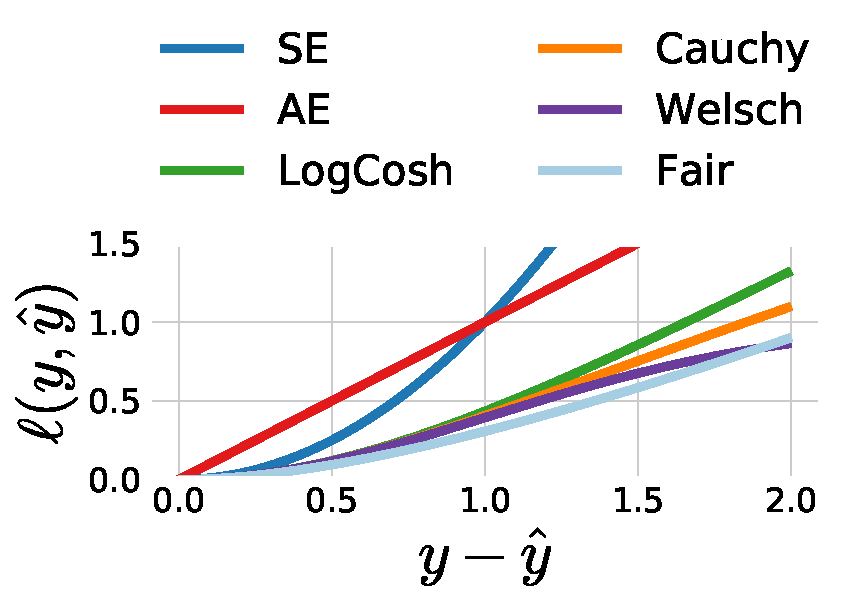
\includegraphics[width=0.98\textwidth]{figures/objective_functions/objective_functions_zoom.pdf}
  \caption[Objective Functions Zoom In]
    {Zoom in of \figref{fig:ml:objective_funcs}. 
    }
  \label{fig:ml:objective_funcs_zoom}
\end{marginfigure}

\begin{figure}
  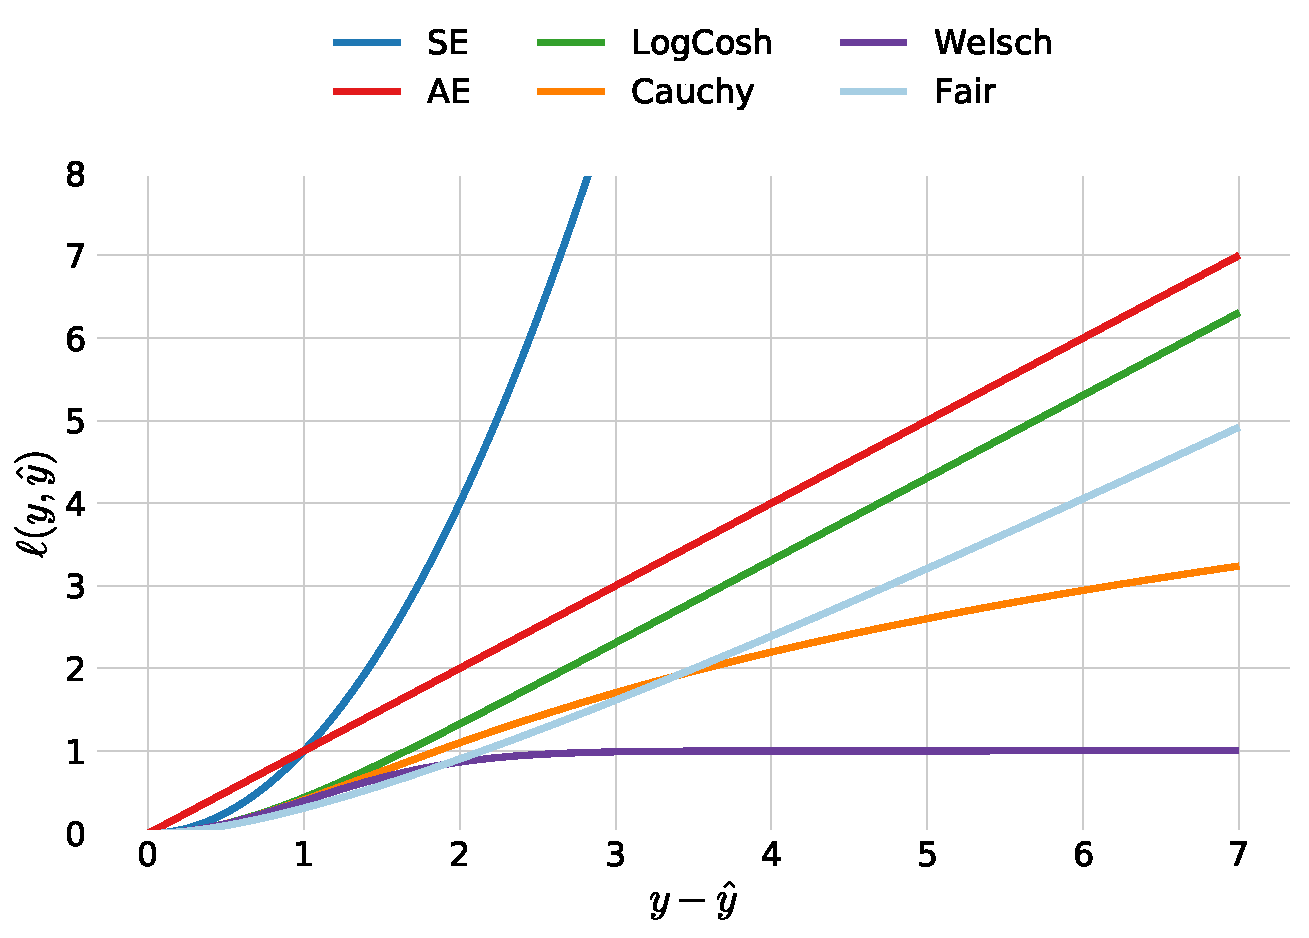
\includegraphics[width=0.9\textwidth]{figures/objective_functions/objective_functions.pdf}
  \caption[Objective Functions]
    {Comparison of the the six loss functions SE, AE, LogCosh, Cauchy, Welsch, and Fair as a function of $y-\hat{y}$, see equation \eqref{eq:ml:loss_functions}. In the plot \textcolor{blue}{SE} is shown in blue, \textcolor{red}{AE} in red, \textcolor{green}{LogCosh} in green, \textcolor{orange}{Cauchy} in orange, \textcolor{purple}{Welsch} in purple, and \textcolor{light-blue}{Fair} in light blue. For the Cauchy, Welsch, and Fair functions $c$ is set to 1. For a zoom in of the inner region 
    where $y-\hat{y}<2$ see \figref{fig:ml:objective_funcs_zoom}. All six graphs are symmetric in $y-\hat{y}$ which is why they are only shown for positive values of $y-\hat{y}$.
    }
  \label{fig:ml:objective_funcs}
\end{figure}


\subsection{Evaluation Function}
Since some machine learning models require an analytic expression for the derivative and second derivative, it not always possible to use a custom objective function if it is non-differentiable. The Area Under Curve (AUC) of the Receiver Operating Characteristic (ROC) is such a measure. Another example would be the width of the distribution of all $y_i-\hat{y}_i$. In this thesis this overall performance metric will be called the \emph{evaluation function} $f_\mathrm{eval}$ compared to the differentiable proxy for this function, the objective function. To sum up: the loss function $\ell(y, \hat{y})$ measures the loss for an individual prediction and the objective function $\mathcal{L}$ is the aggregated version of the individual losses. The objective function is assumed to be a good proxy for the evaluation function $f_\mathrm{eval}$ which is the overall metric.  
For the loss functions defined in \autoref{sec:ml:loss_function} the objective function is based on the mean of the individual losses:
\begin{equation}
  \mathcal{L} = \frac{1}{N} \sum_{i=1}^N \ell(y_i, \hat{y}_i) + \Omega. 
\end{equation}

\section{Decision Trees}
\label{sec:ml:decision_trees}

\begin{marginfigure}
  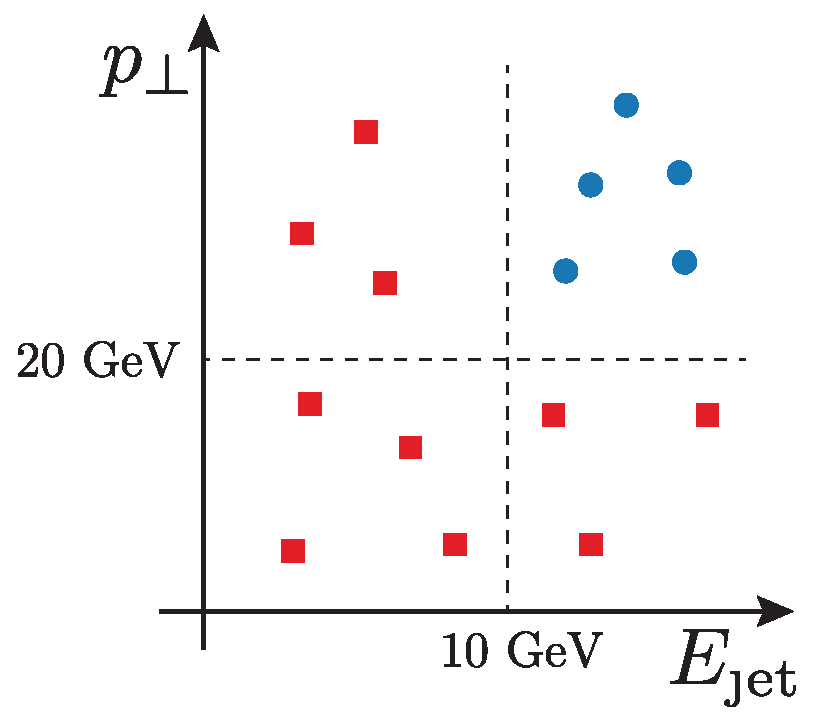
\includegraphics[width=0.99\textwidth, trim=10 10 10 10, clip]{figures/decision_tree/tree_example.pdf}%     without .tex extension
  % or use \input{mytikz}
  \caption[Decision Tree Cuts In Feature Space]{Illustration of the cuts a decision tree model make for \textcolor{blue}{signal} in blue circles and \textcolor{red}{background} in red squares. This is an visualization in the feature space of the decision tree seen in Figure~\ref{fig:ml:decision_tree}.}
  \label{fig:ml:decision_tree_feature_space}
\end{marginfigure}

Decision Trees are a simple machine learning method that works by partitioning the feature space into smaller subspaces, high-dimensional rectangles basically, and then fit each subspace with a constant for regression problems or a single label for classification problems \citep{hastieElementsStatisticalLearning2009}. A simple example of this can be seen in Figure~\ref{fig:ml:decision_tree_feature_space} and Figure~\ref{fig:ml:decision_tree}. In the first figure we see an illustration of how the signal and background distributions look in the 2D feature space. The dashed lines in the figure indicate the cuts made by the decision tree (DT), cuts which are shown on the second figure as a typical DT plot. 
\begin{figure}
  \centering
  \includestandalone[width=0.6\textwidth]{figures/decision_tree/decision_tree}%     without .tex extension
  % or use \input{mytikz}
  \caption[Decision Tree]{
    Illustration of a simple decision tree. Here the tree partitions the input feature space consisting of the two variables $p_\perp$ and $E_\mathrm{jet}$ into two categories; either signal or background. A visualization of the cuts in the feature space can be seen in Figure~\ref{fig:ml:decision_tree_feature_space}.
  }
  \label{fig:ml:decision_tree}
\end{figure}
Here the top \q{box} is called the \emph{root} of the tree, any subsequent boxes are \emph{nodes} except the final ones that are not split any further which are \emph{leaves}.

At first the decision tree partitions the space according to the value of the transverse momentum\sidenote{All units in this project are in natural units such that both momentum and energy are in units of \si{\eV}.} $p_\perp$: if it is lower than (or equal to) \SI{20}{\GeV} then it classified as background. If the value is higher than \SI{20}{\GeV} then an extra split is made, this time on the energy of the jet $E_\mathrm{jet}$: if it is higher than \SI{10}{\GeV} it is classified as signal and otherwise as background. Training a DT on this data allows us to predict a new unseen event $(p_\perp, E_\mathrm{jet}) = (\SI{24}{\GeV},\SI{11}{\GeV})$ to be a signal-like event. This DT is said to be a shallow tree since it only has a depth of \num{2}. The maximum depth allowed for the model is an important hyperparameter since it clearly controls under- and overfitting by changing how many cuts and partitions in the feature space are allowed; the deeper the tree, the more complex the model becomes. Single DTs are very prone to overfitting
% \sidenote{With a solution to this problem given in \autoref{subsec:ml:multiple_decision_trees}.}
, however, they are also extremely inspectable. They are even referred to as \q{white-box models} compared to black-box models such as neural networks. For a more thorough introduction to decision trees and how they are internally optimized (for finding the best cut values), see \citet{hastieElementsStatisticalLearning2009}. 

\subsection{Ensembles of Decision Trees}
\label{subsec:ml:multiple_decision_trees}
Single decision trees are prone to overfitting and generally suffer from high variance. Today especially two different methods exist to alleviate these problems: Random Forests (RFs) and Boosted Decision Trees (BDTs). Both methods are examples of so-called ensemble methods where a set of ML methods are combined into a single model. Typically ensemble methods are based on \emph{weak learners}: simple, often fast, methods that individually show relatively poor generalization performance typically due to high variance. 

\subsubsection{Random Forests}
\label{subsubsec:ml:random_forest}
Random Forests were first introduced in 2001 by \citet{breimanRandomForests2001}. Random Forests are a collection of $B$ decision trees where each tree is trained on bootstrapped versions of the training data and then the individual trees' predictions $T_b$ are averaged\sidenote{In the case of classification it is the majority vote which is taken.}: 
\begin{equation}
  f_\mathrm{RF}(\vec{x}) = \hat{y}_\mathrm{RF} = \frac{1}{B}  \sum_{b=1}^B T_b(\vec{x}).
\end{equation}
The method of making artificial extra samples and training on them is in general called bootstrap aggregation or \emph{bagging} \autocite{hastieElementsStatisticalLearning2009}. It works by averaging out noisy estimates of the individual models hence reducing variance. 
\begin{theorem}[Variance of average of correlated i.d. variables]
  Given $B$ identically distributed (but not necessarily independent) variables each with variance $\sigma^2$ and positive pairwise correlation $\rho$, the variance of the average is:
  \begin{equation}
    \label{eq:ml:variance_of_correlated_variables}
    \mathrm{Var}(\bar{\mu}_B) = \frac{1-\rho}{B} \sigma^2 + \rho \sigma^2,
  \end{equation}
  where $\bar{\mu}_B$ is the average of the i.d. variables \autocite{hastieElementsStatisticalLearning2009}. % XXX maybe write proof here myself: https://stats.stackexchange.com/questions/320083/calculating-the-variance-of-the-average-of-b-dependent-random-variable
\end{theorem}
Equation \eqref{eq:ml:variance_of_correlated_variables} is the main idea behind RFs. As the number of trees $B$ in the forest increases, the first term goes towards zero. Thus, the more the correlation $\rho$ between the individual trees is reduced, the more the variance is reduced (which is the main problem in the case of DTs to begin with). 

In addition to training the trees on bagged samples, one more technique is used to further decrease the correlation between the individual trees: each bootstrapped sample of the dataset not only contains just a subset of the observations (rows), but also only a subset of the variables (columns)\sidenote{Throughout this project all data is assumed to be \emph{tidy data} unless otherwise explicitly mentioned. Tidy data was a concept formalized in 2003 by \citet{JSSv059i10} which basically states that each variable forms a columns, each observation forms a row, and that each type of observation unit forms a table. This also means that the term variable and column will be used interchangeable (together with \emph{feature}), and likewise with observation and row.}. This is called column-subsampling (in contrast to row subsampling).

% Until very recently RF has suffered from the lack of a fast, optimized implementation in Python that could deal with big data sets. 

\subsubsection{Boosted Decision Trees}
\label{subsubsec:ml:boosted_decision_trees}
In the overall family of ensemble models, \emph{boosting} might be the most successful of them all where especially the specific algorithm called XGBoost \autocite{chenXGBoostScalableTree2016} revolutionized the ML world by winning numerous Kaggle\sidenote{Kaggle is an online platform where people compete with machine learning models.} competitions \autocite{DmlcXgboost} including the Higgs Machine Learning competition in \num{2014} \autocite{HEPMeetsML}. 

Boosting is the process of sequentially applying weak learner models to repeatedly modified versions of data \autocite{hastieElementsStatisticalLearning2009}. In an iterative fashion this combines many weak learners into a single strong learner. The final prediction is thus a weighted sum over the $K$ different weak learners $F_k$: 
\begin{equation}
  f_\mathrm{BDT}(\vec{x}) = F(\vec{x}) = \sum_{k=1}^K \alpha_k F_k(\vec{x})
\end{equation}
Boosting thus works by reducing both bias and variance since it iteratively fits weak learners. The variance is not reduced as much as for RFs since the weak learners are more correlated, however, their bias is lower. 

The term gradient boosting comes from the observation that repeatedly minimizing the residuals of the current model is similar to minimizing the gradient of the loss function for a specific choice of the loss function.

Imagine that we start off with an imperfect model $F_k(x)=\hat{y}$. In boosting we want the next iteration to be a better model than the previous one, so imagine that the perfect addition to the model that we needed to make was $h(x)$. For it to be perfect, the following would have to be true:
\begin{equation}
  \label{eq:ml:boosted_decision_trees_residual}
  F_{k+1}(x) = F_k(x) + h(x) = y \Leftrightarrow h(x) = y - F_k(x).
\end{equation}
The r.h.s. is the residual of the model, so at each stage the model is trying to fit the residuals of the current iteration of model. The \q{gradient} in \q{gradient boosting} comes from the following. Assume the loss function: $L(y, F_k(x)) = \frac{1}{2}  (y-F_k(x))^2$. The gradient of the loss w.r.t. to $F_k(x)$ is:
\begin{equation}
  \frac{\partial L(y, F_k(x))}{\partial F_k(x)} = F_k(x) - y. 
\end{equation}
This is exactly the negative of the r.h.s. of equation \eqref{eq:ml:boosted_decision_trees_residual}. Instead of looking at the model as trying to minimize the residual at each iteration, it can instead be generalized as trying to fit the negative gradients of the loss function:
\begin{equation}
  h(x) = - \frac{\partial L}{\partial F_k}.
\end{equation}
We thus end up with the following iterative model which is basically a \emph{gradient descent} algorithm.
\begin{equation}
  F_{k+1}(x) = F_k(x) + h(x) = F_k - \frac{\partial L}{\partial F_k}.
\end{equation}


AdaBoost \autocite{freundDesiciontheoreticGeneralizationOnline1995} was the first major algorithm to make use of boosting. It was seen as a way of iteratively giving wrongly predicted observations higher weight, however, this is just a result of a \q{lucky} choice of loss function\sidenote{Exponential loss for classification.} which was not realized until much later. AdaBoost could be used with many different weak learners, however, mostly DTs were used to form BDTs. XGBoost \autocite{chenXGBoostScalableTree2016} is a fast, computationally efficient implementation of gradient boosting with DTs as base learners. It implements several model regularization techniques which makes it less prone to overfitting than other BDTs. 

\section{Hyperparamater Optimization}
\label{sec:ml:hyperparameter_optimization}
By now linear models with $L_1$ and $L_2$ regularization have been introduced along with decision trees (DTs), random forests (RFs) and gradient boosted trees (GBTs). All of these ML models tries to optimize their parameters according to some objective function. In addition to the parameters of the model, each one has a specific set of hyperparameters that cannot directly be optimized in the internal optimization process. This could be the amount of regularization $\lambda$ for linear models, the maximum tree depth for DTs, the number of trees for RFs, or the column (or row) subsampling fraction for BTDs. 

In general we say that we have the ML model $\mathcal{A}$ with $K$ hyperparameters. Each of these hyperparameters have a domain $\Lambda_k$. The domain can be either real numbers $\Lambda_k \in \mathbb{R}$, integers $\Lambda_k \in \mathbb{Z}$, binary $\Lambda_k \in \{0, 1\}$, or categorical\sidenote{Could e.g. be the choice of loss function.}. We define the hyperparameter configuration space as: $\bm{\Lambda} = \Lambda_1 \times \Lambda_2 \times \dots \times \Lambda_K$. Within this space we are searching for a vector of hyperparameters $\bm{\lambda} \in \bm{\Lambda}$ which defines the optimal model $\mathcal{A}_{\bm{\lambda}^*}$. Here the optimal model is the defined as the model which gives the best generalization performance according to some evaluation function. The goal of finding the best hyperparameter $\bm{\lambda^*}$ is known as \emph{hyperparameter optimization} (HPO.)

The first naive approach would simply to manually\sidenote{Also known jokingly as \q{Grad Student Descent}.} try out different combinations of $\bm{\lambda}$ and see performance on the validation set\sidenote{Remember only to use the test set on the final model.}. This is of course too cumbersome for advanced ML models, but it should be noted that it is a good place to start. In \autoref{subsec:ml:grid_search} the HPO method called Grid Search is introduced which is further generalized and optimized in \autoref{subsec:ml:random_search} with Random Search. Both these methods are easily parallelizable since they do not have any inherent history in its guesses. This is in contrast to Bayesian Optimization introduced in \autoref{subsec:ml:bayesian_optimization} which allows for \q{smart} guesses.

\subsection{Grid Search}
\label{subsec:ml:grid_search}

Grid search (GS) is a HPO method also known as full factorial design. It is called this because it tries out all possible combinations of the hyperparameter configuration space: the so-called cartesian product of $\bm{\Lambda}$. Imagine a 2D space where the two domains are respectively $x=\{1, 2, 3\}$ and $y=\{1, 2, 3,4\}$. Then GS runs through all $3 \times 4 = 12$ combinations of these two sets: 

\begin{marginfigure}
  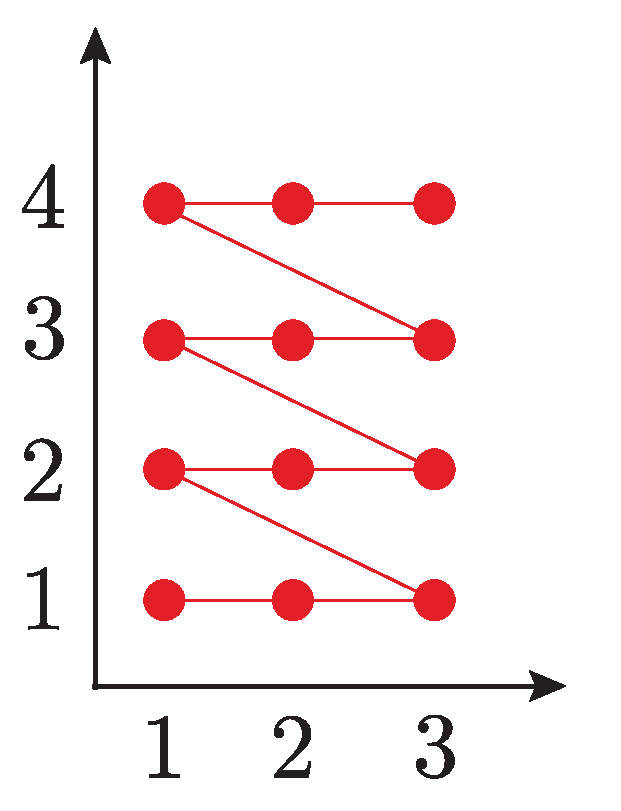
\includegraphics[width=0.8\textwidth]{figures/gridsearch/grid.pdf}
  \caption[Grid Search]{Visualization of grid search run on the two hyperparameters $x$ and why $y$ with the domains $x=\{1, 2, 3\}$ and $y=\{1, 2, 3,4\}$.}
  \label{fig:ml:gridsearch}
\end{marginfigure}

\begin{equation}
  (x_i, y_i) \in \{(1, 1), (1, 2), \dots, (x_i, y_i), \dots, (3, 4)\},
\end{equation}
as visualized in Figure~\ref{fig:ml:gridsearch}. The advantage of GS is that it is an exhaustive search over all combinations\sidenote{Note that the user has to provide the values for each hyperparamater to be tried out manually.} of hyperparameters, however, the total number of combinations grows exponentially and GS as a method thus suffers the curse of dimensionality\sidenote{Not the dimensionality of the input feature space, but of the hyperparameter configuration space.}.



\subsection{Random Search}
\label{subsec:ml:random_search}

To circumvent the problems of grid search, \citet{bergstraRandomSearchHyperparameter2012} developed the Random Search (RS) algorithm in 2012. Regarding the effect of the curse of dimensionality on grid search they wrote: \emph{``This failure of grid search is the rule rather than the exception in high dimensional hyper-parameter optimization''} \citep{bergstraRandomSearchHyperparameter2012}. Instead of searching through all possible values of $\bm{\lambda}$ like in GS, RS makes $B$ runs where each $\bm{\lambda}_i$ is given by:
\begin{equation}
  \label{eq:ml:random_search}
  \bm{\lambda}_i \sim \sum_{j=1}^K  \mathrm{PDF}_j(\Lambda_j) \cdot \bm{\hat{e}}_j  .
\end{equation}
Equation \eqref{eq:ml:random_search} should be understood in the following way. For each hyperparameter draw a random number from a user-defined Probability Density Function (PDF) and then let $\bm{\lambda}$ be the vector of those $N$ random numbers. In a 2D-space $\bm{\lambda}_i$ could thus be: 
\begin{align}
  \bm{\lambda}_i \sim &= \begin{bmatrix}
      \mathcal{N}(100, 4) \\
      \mathcal{U}(0, 1)
       \end{bmatrix},
\end{align}
where $\mathcal{N}(100, 2)$ is normal (Gaussian) distribution with mean $\mu=100$ and standard deviation $\sigma^2=4$ and $\mathcal{U}(0, 1)$ is the uniform distribution in the interval $[0, 1]$. Of course the PDF can be a PMF in the case of discrete hyperparameter domains.

\begin{marginfigure}
  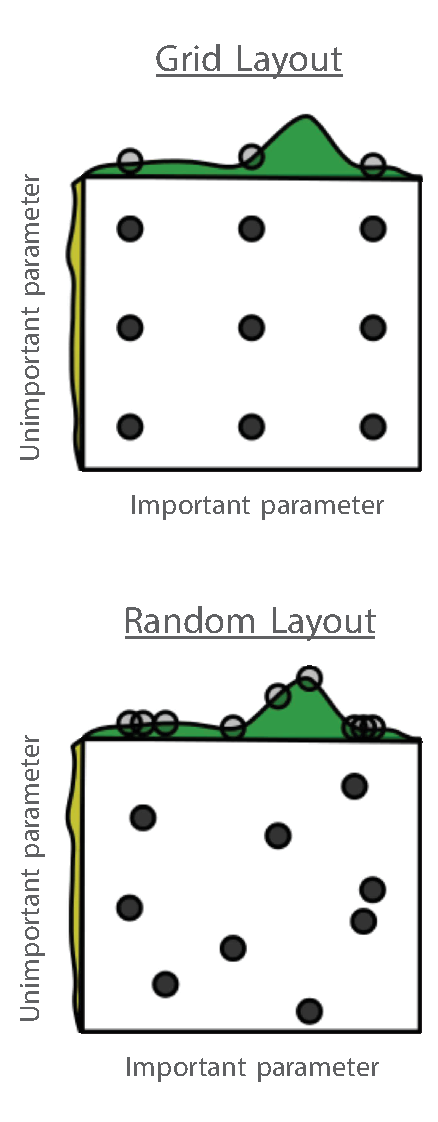
\includegraphics[width=0.8\textwidth]{figures/randomsearch/random.pdf}
  \caption[Random Search]{Visualization of the difference between grid search and random search. Adapted from \citet{bergstraRandomSearchHyperparameter2012}.}
  \label{fig:ml:random_search}
\end{marginfigure}

The reason why random search is so powerful is not only because the number of function evaluations $B$ is easily tunable\sidenote{Compared to grid search which tries \emph{all} possible combinations.}, but also due to the fact that often some hyperparameter dimensions are more important than other. Even though the hyperparameter configuration space $\bm{\Lambda}$  might be high-dimensional, it often exhibits \emph{low effective dimensionality} \autocite{bergstraRandomSearchHyperparameter2012}. In the simplest 2D-case this can be written as the following example. Imagine that we want to maximize some evaluation function, e.g. accuracy of the predictions, and the model depends on the two independent hyperparameters $x$ and $y$: $f(x, y)$. In this example assume that $f$ is almost insensitive to $y$ and thus has an effective dimensionality of 1. Then $f(x,y) = g(x) + h(y) \approx g(x)$. For a visualization of this example, see Figure~\ref{fig:ml:random_search}.

Here GS is run with a grid of $3\times3 = 9$ points and RS is similarly run with 9 points drawn from uniform PDFs in the same interval. It easy to see that when the hyperparameter configuration space has a lower effective dimensionality than the actual dimensionality RS is far better at probing the space due to the projections into the sensitive dimensions cover more of these axes than for GS. In general in ML the hyperparameter configuration space has lower effective dimension than its actual dimension, but different hyperparameters matter in different datasets

In general only a fraction of all hyperparameters matter for any dataset but different hyperparameters matter in different datasets and thus generally RS performs as well as GS or better \autocite{bergstraRandomSearchHyperparameter2012}. 

Note that RS can be seen as a generalization of GS, where GS is the specific example of RS if one uses a multidimensional binomial distribution as PDF where the PDF is reevaluated after each run. 

\subsection{Bayesian Optimization}
\label{subsec:ml:bayesian_optimization}
When performing hyperparameter optimization it often takes a lot of time to evaluate the individual hyperparameters. Remember, that each evaluation consists of fitting $\mathcal{A}_{\bm{\lambda}}$ to the training data and then measure the performance on the validation set. Fitting the model on the training set can often take minutes, if not hours. This process is even slower when using cross validation. The idea behind Bayesian Optimization is that when the ML model, or any other black box function, is expensive\sidenote{With respect to time.} to evaluate then \q{smart} guesses are worth spending a bit of time on developing. The hope is that the time taken to come up with smart guesses is negligible compared to the overall function evaluation time. This is contrast to both GS and RS where each new set of hyperparameters $\bm{\lambda}$ is independent of the value of the evaluation performance.

In Bayesian Optimization (BO) \autocite{brochuTutorialBayesianOptimization2010}, the evaluation function as a function of hyperparameter is unknown. This unknown function is iteratively fitted with a probabilistic surrogate model, most often by Gaussian processes (GPs). Given the fitted surrogate model, an acquisition function is computed. This is a manually chosen function which is cheap to evaluate and is a measure of where in the hyper-dimensional hyperparameter space there is a highest chance of finding a new good value of $\bm{\lambda}$. The acquisition function has to be chosen manually and especially the tradeoff between \emph{exploitation} versus \emph{exploration} is particularly important. This value decides how \q{adventurous} or conservative the BO algorithm should be when exploring the evaluation space. 

Bayesian Optimization is better explained by looking at Figure~\ref{fig:ml:bayesian_optimization}. First look at the top plot. This is a plot of the surrogate function in black with uncertainties shown in blue. This is a result of fitting GPs to the two previous points in black, $t=2$. This surrogate function is supposed to fit the unknown hyperparameter-dependent evaluation function (called objective in the figure) shown as a dashed black line. Below we see the acquisition function in green. This is a function of the blue curve and the position of its maximum decides where the next guess of $\bm{\lambda}$ should be. With the chosen acquisition function and exploration willingness, we see that the next guess should be slightly to the left of the right-most point. This is a simple 1D toy problem, but one should imagine this happening in a high-dimensional space. After making a new guess, $t=3$ in the middle plot, the acquisition function changes since it learnt that this gave a worse evaluation value than the right-most point. Therefore, the next proposal for $\bm{\lambda}$ is slightly to the right of the right-most point. The process continues like this in an iterative fashion: first fitting GPs to the previous evaluation values and then choosing the next $\bm{\lambda}$ according the acquisition function given the GPs. 

\begin{marginfigure}[-2cm]
  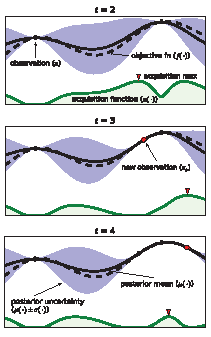
\includegraphics[width=0.99\textwidth]{figures/bayesian_optimization/bo.pdf}
  \caption[Bayesian Optimization]{Illustration of the learning process of Bayesian optimization. The previous observations are shown as black dots and the true objective function is shown as a dashed black line. This line is fitted with Gaussian processes (GPs) which is shown as the solid line with its uncertainty in purple. The acquisition function is shown in green and its maximum decides what the next iteration of the hyperparameter value(s) should be. 
  Adapted from \citet{brochuTutorialBayesianOptimization2010}.}
  \label{fig:ml:bayesian_optimization}
\end{marginfigure}

Gaussian Processes provide a posterior distribution given some prior distribution and the data-dependent likelihood. The process of BO is quite technical and mathematical, especially if GPs are new material. For a more in-depth explanation of the topic, see \citet{brochuTutorialBayesianOptimization2010}. The important thing to note is that GPs return not only a posterior mean $\mu(\vec{x})$ but also an uncertainty $\sigma(\vec{x})$, as seen in Figure~\ref{fig:ml:bayesian_optimization} described above. The acquisition function used in this project is the Upper Confidence Bound (UCB):
\begin{equation}
  \mathrm{UCB}(\vec{x}) = \mu(\vec{x}) + \kappa \sigma(\vec{x}),
\end{equation}
where $\kappa \geq 0$ is the parameter\sidenote{Here $\kappa$ can be regarded as a hyper-hyperparameter since it controlls how the other hyperparamaters are optimized.} controlling the exploration-exploitation tradeoff. 

Bayesian Optimization has the great benefit of slowly learning the hyperparameter space and making smarter and more educated guesses over time. However, it also comes with the cost of being harder to numerically implement compared to GS and RS\sidenote{Which are basically plug-and-play with Scikit-Learn \autocite{scikit-learn}.}, and parallelization is non-trivial to implement since it by definition is a sequential process. The performance boost is also not guaranteed. 

\section{Feature Importance}
\label{sec:ml:feature_importance}
Having first established in \autoref{sec:ml:supervised_learning} that machine learning algorithms are indeed able to not only learn from data but also to generalize well without overfitting (\autoref{sec:ml:overfitting}), modern ML algorithms such as decision trees, random forests and boosted decision trees were introduced in \autoref{sec:ml:decision_trees} and they were hyperparameter optimized in \autoref{sec:ml:hyperparameter_optimization}, one would expect that one would have a well performing model by now. 

Now comes one of the most important issues in ML today: model inspection. Actually trying to make sense of the learnt model. Why does it predict as it does? Which features or variables are most important according to the model? Model interpretation is still very much active research today with no universally accepted methods. Some methods are model dependent and accurate, others might be model agnostic but slow or only approximations. In this project the focus will be on the so-called \emph{SHAP} values. 

In 2017 \citet{Lundberg:2017} showed that six different previously used methods were all specific instances of a universal underlying method\sidenote{The class of \emph{additive feature attribution methods} \citep{Lundberg:2017}.} and proposed SHaplay Additive exPlanation (SHAP) values as a unified measure of feature importance. In \num{2018} they developed a fast algorithm for computing SHAP values for tree ensemples and showed that previous measures of feature importance heavily used for trees, e.g. \emph{gain}, were \emph{inconsistent} \autocite{lundbergConsistentIndividualizedFeature2019}. That a measure for feature importance is inconsistent means that a model could rely more on feature $A$ than $B$, however, the feature importance would indicate opposite. SHAP values and \emph{permutation}-based feature importances are both consistent feature importance measure, however, only SHAP allows for individualized\sidenote{Meaning that you can get the feature importances for a single observation compared to only the global, overall feature importances as seen across the entire data set.}, or local, feature importances.  

SHAP values are within the class of additive feature attribution methods, which are functions where the explanation model $g$ is a linear combination of binary variables:
\begin{equation}
  \label{eq:ml:additive_feature_attribution_method}
  g(z') = \phi_0 + \sum_{i=1}^M \phi_i z_i'.
\end{equation}
Here $\phi_i \in \mathbb{R}$ are the feature importances and $z'$ is a binary variable such that $z_i'=1$ if the feature is present and otherwise $z_i' = 0$. SHAP values are based on Shapley regression values known from cooperative game theory \autocite{Shapley1953}. These values are based on the three axioms:
\begin{axiom}[Local Accuracy]
  Local accuracy says that the sum of the feature importances should equal the total reward:
  \begin{equation}
    f(x) = g(z') = \phi_0 + \sum_{i=1}^M \phi_i z_i'.
  \end{equation}
\end{axiom}
Here $f$ is the ML model, $g$ is the explanation model, $x$ is an observation in input feature space, $z'$ is an observation in the binary space as described above, and $\phi_i$ is the feature importance. 
\begin{axiom}[Missingness]
  Missingness means that features missing in the original input feature space (such that $z_i'=0$) should be attributed no importance:
  \begin{equation}
    z_i' = 0 \Rightarrow \phi_i = 0.
  \end{equation} 
\end{axiom}
\begin{axiom}[Consistency]
  \label{axiom:ml:shap_consistency}
  Consistency states if a model is changed such that it relies more on a certain feature, the feature importance of that feature should never decrease. 
\end{axiom}
% \begin{description}
%   \item[Local Accuracy] 
%   Local accuracy says that the sum of the feature importances should equal the total reward:
%   \begin{equation}
%     f(x) = g(x') = \phi_0 + \sum_{i=1}^N \phi_i x_i'.
%   \end{equation}
%   Here $f$ is the ML model, $g$ is the explanation model, $x$ is an observation in input feature space, $x'$ is an observation in the binary space as described above, and $\phi_i$ is the feature importance. 

%   \item[Missingness] Missingness means that features missing in the original input feature space (such that $x_i'=0$) should be attributed no importance:
%   \begin{equation}
%     x_i = 0 \Rightarrow \phi_i = 0
%   \end{equation}
%   \item[Consistency] Consistency states if a model is changed such that it relies more on a certain feature, the feature importance of that feature should never decrease.
% \end{description}
Given these three axioms, \citet{Lundberg:2017} show that the only solution to equation \eqref{eq:ml:additive_feature_attribution_method} is:
\begin{equation}
  \label{eq:ml:shap_feature_importance}
    \phi_i = \sum_{S \subseteq \widetilde{M} \backslash \{i\}} \frac{|S|!(M-|S|-1)!}{M!} \left[ f_x(S \cup \{i\}) - f_x(S) \right] ,
\end{equation}
which one can simplify to:
\begin{equation}
  \label{eq:ml:shap_feature_importance_simplification}
  \begin{split}
    \phi_i        &= \sum_{S \subseteq \widetilde{M} \backslash \{i\}} w(S) \cdot \Delta_{f_x}(S) \\
    w(S)             &\equiv \frac{|S|!(M-|S|-1)!}{M!} \\
    \Delta_{f_x}(S)  &\equiv \left[ f_x(S \cup \{i\}) - f_x(S) \right].
  \end{split}
\end{equation}


In equation \eqref{eq:ml:shap_feature_importance} $\widetilde{M}$ is the \emph{set} of all input features\sidenote{Compared to $M=|\widetilde{M}|$ which is the \emph{number} of all input features.}, $S \subseteq \widetilde{M} \backslash \{i\}$ means a subset $S$ of $\widetilde{M}$ without feature $i$, $S \cup \{i\}$ means the set $S$ with feature $i$ and $f_x(S) = f(h_x(z'))$ where $h_x(z')$ is the mapping function from the binary $z'$ space to the input feature space $x$. In equation \eqref{eq:ml:shap_feature_importance_simplification} the function is simplified to its basic constituents: the difference in performance  between including feature $i$ and not including it, $\Delta_{f_x}$, and its weight $w$. 

To get a better understanding of the different sets in the summation, one could look at the decision tree shown in Figure~\ref{fig:ml:decision_tree}. Here $\widetilde{M}$ would be $\widetilde{M}=\{p_\perp, E_\mathrm{jet} \}$. For the feature $i=p_\perp $ one would thus have:
\begin{equation}
  \begin{split}
    \phi_{p_\perp} = & \sum_{S \subseteq \widetilde{M} \backslash \{p_\perp \}} w(S)  \cdot\Delta_{f_x}(S)  \\
                   = & \sum_{S \in \left[\{\}, \{E_\mathrm{jet}\} \right]} w(S)  \cdot\Delta_{f_x}(S)  \\
                   = & \frac{0! (2-0-1)!}{2!} \cdot [ f_x(\{p_\perp\}) - f_x(\{\})]  \\ 
                     & +    \frac{1! (2-1-1)!}{2!} \cdot [f_x(\{ E_\mathrm{jet}, p_\perp \}) - f_x(\{ E_\mathrm{jet} \})].
  \end{split}
\end{equation}
Whereas $w(S)$ are easily calculated, $\Delta_{f_x}$ depends on the data. As the number of features grows, the number of terms in the sum grows exponentially. What \citet{lundbergConsistentIndividualizedFeature2019} did was to develop an efficient algorithm that could solve this for trees in polynomial time\sidenote{Specifically they managed to improve the time complexity from $\mathcal{O}(TL2^M)$ to $\mathcal{O}(TLD^2)$ where $T$ is the number of trees, $L$ is the maximum number of leaves in any tree, $M$ is the number of features, and $D$ is the maximum depth of any tree (where $D\approx \log L$ for balanced trees).}. 

SHAP values allows one to explain for a single prediction why it got the prediction that it got. When applied to the entire data set $\vec{X} \in \mathbb{R}^{N \times M}$ with $N$ observations each with $M$ features, one gets the matrix $\bm{\Phi}$. When summing over the absolute value of each column, one gets the global impact $\phi_i^\mathrm{tot}$ of the $i^{\mathrm{th}}$ feature \citep{lundbergConsistentIndividualizedFeature2019}:
\begin{equation}
  \phi_i^\mathrm{tot} = \sum_{j=1}^N \abs{ \bm{\Phi}_{i, j} }.
\end{equation}
The global feature importance $\phi_i^\mathrm{tot}$ is thus a measure of the overall importance of feature $i$. 

Note that if one introduces a new feature to the dataset correlated\sidenote{Not necessarily linearly correlated.} to an already existing feature, the feature importance of the previous feature will decrease. 
This is due to the axiom of symmetry:
\begin{axiom}[Symmetry]
  \label{axiom:ml:shapley_symmetry}
  If for all subsets S that do not contain $i$ or $j$: 
  \begin{equation}
    f_x(S \cup \{i\}) = f_x(S \cup \{j\})
  \end{equation}
  then $\phi_i = \phi_j$.
\end{axiom}
It can be shown that axiom \ref{axiom:ml:shapley_symmetry} is implied by axiom \ref{axiom:ml:shap_consistency}  \citep[Supp. Material]{Lundberg:2017}. Two identical features, as seen by the model, will thus \q{share} the feature importance.
